\section{Results}
\label{sec:results}

We organize the results around five hypotheses. H1: at least 95\% of prompts give identical outputs across batch sizes. H2: divergence grows with output length. H3: math and reasoning diverge more than classification. H4: mean accuracy changes by less than 1\pp while individual items flip. H5: smaller models diverge more. \Tabref{tab:verdicts} in \secref{sec:discussion} summarizes the verdicts.

\subsection{How often do greedy outputs change?}
\label{sec:res_rate}

\begin{table}[t]
    \centering
    \caption{Percentage of prompts whose greedy output is \emph{not} token-identical between two conditions, shown as long (CoT, $n=700$) / short (label, $n=1000$). For the 3B bf16 models, comparisons against \bone use the 140/200-item subsets, and \cond{b4} was not run (--). Repeats are exactly zero everywhere. Reshuffling batch-mates at fixed $B=64$ gives almost the same divergence as going from $B=1$ to $B=64$. Lowest (most stable) values per column in \textbf{bold}.}
    \label{tab:divergence}
    \resizebox{\textwidth}{!}{%
    \begin{tabular}{@{}llcccccc@{}}
        \toprule
        & & \multicolumn{3}{c}{\textbf{Batch size vs.\ $B=1$}} & \multicolumn{3}{c}{\textbf{Controls}} \\
        \cmidrule(lr){3-5} \cmidrule(lr){6-8}
        \textbf{Model} & \textbf{dtype} & \bone vs \cond{b4} & \bone vs \cond{b16} & \bone vs \bsf & \bsf vs \bshuf & \bsf vs \brep & \bone vs \cond{b1\_rep} \\
        \midrule
        \qwen-0.5B & bf16 & 75.9 / 3.6 & 75.0 / 3.7 & 76.4 / 3.4 & 72.7 / 1.3 & 0 / 0 & 0 / 0 \\
        \qwen-1.5B & bf16 & 45.1 / 1.9 & 44.0 / 1.1 & 46.9 / 1.1 & 40.0 / 0.3 & 0 / 0 & 0 / 0 \\
        \qwen-3B   & bf16 & --          & 65.7 / 2.5 & 76.4 / 3.0 & 63.7 / \textbf{0.0} & 0 / 0 & -- \\
        \llama-1B  & bf16 & 50.1 / 2.3 & 50.1 / 4.3 & 51.7 / 4.1 & 45.3 / 0.4 & 0 / 0 & 0 / 0 \\
        \llama-3B  & bf16 & --          & 57.1 / 1.0 & 54.3 / 1.5 & 47.0 / 0.4 & 0 / 0 & 0 / 0 \\
        \midrule
        \qwen-0.5B & fp16 & 17.9 / 0.5 & 20.7 / 0.4 & 17.3 / 0.3 & 16.1 / \textbf{0.0} & 0 / 0 & 0 / 0 \\
        \qwen-0.5B & fp32 & \textbf{6.1} / 0.3 & 7.4 / 0.3 & \textbf{6.3} / 0.4 & \textbf{4.9} / \textbf{0.0} & 0 / 0 & 0 / 0 \\
        \midrule
        \qwen-0.5B & AWQ  & 18.4 / 0.4 & 18.0 / 0.3 & 20.1 / 0.2 & 19.9 / 0.4 & 0 / 0 & -- \\
        \qwen-1.5B & AWQ  & 7.9 / 0.2  & \textbf{6.0} / 0.1 & 7.4 / 0.3 & 8.7 / 0.1 & 0 / 0 & 0 / 0 \\
        \qwen-3B   & AWQ  & 15.0 / \textbf{0.0} & 14.4 / \textbf{0.0} & 13.6 / \textbf{0.0} & 13.9 / \textbf{0.0} & 0 / 0 & 0 / 0 \\
        \bottomrule
    \end{tabular}
    }
\end{table}


\begin{figure}[t]
    \centering
    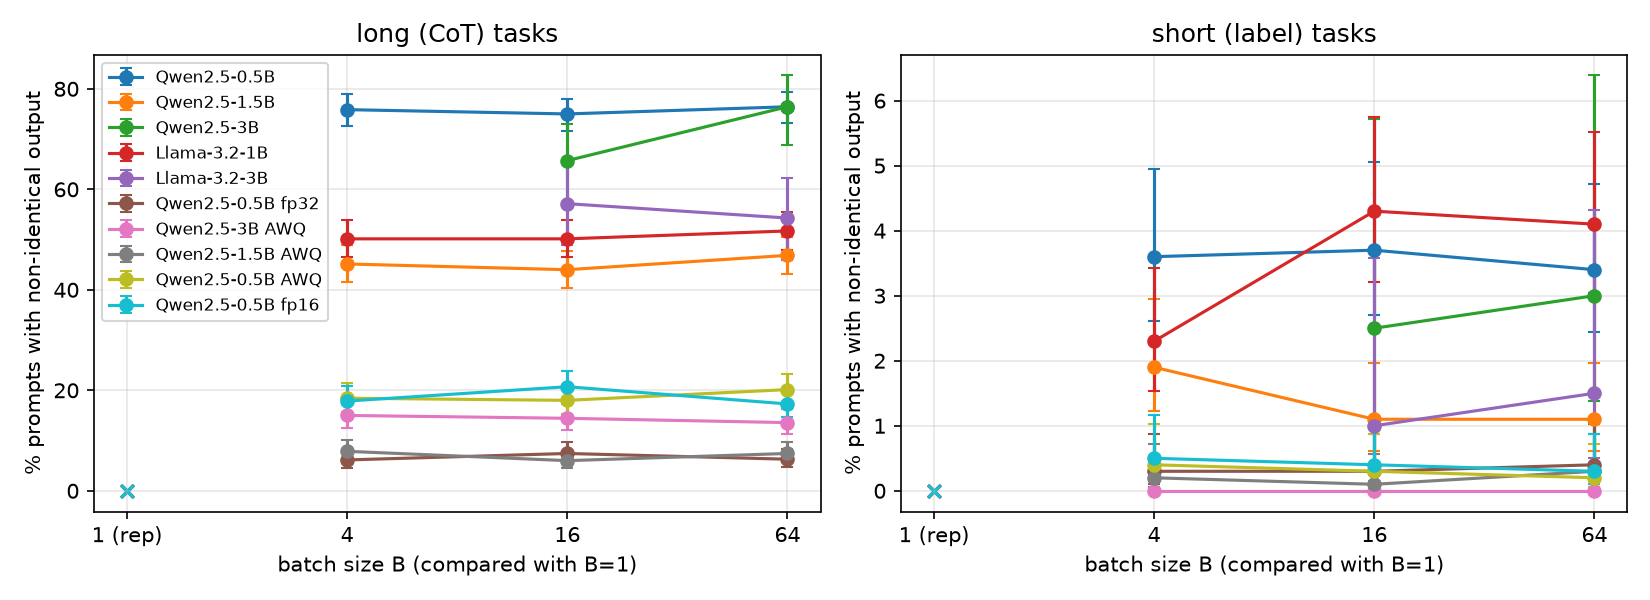
\includegraphics[width=0.95\linewidth]{figures/divergence_vs_batch.png}
    \caption{Share of prompts whose output differs from the sequential ($B=1$) run, for long CoT tasks \figleft and short label tasks \figright. Error bars are Wilson 95\% CIs; ``1 (rep)'' is the $B=1$ repeat, which never diverges. bf16 models (top five lines in the left panel) diverge on 45--76\% of CoT prompts already at $B=4$, and the rate does not grow with $B$. fp16, fp32 and AWQ configurations sit far lower.}
    \label{fig:batch}
\end{figure}

{\bf H1 is refuted for bf16.} Pooled over all 1,700 prompts, the share of outputs that change between $B=1$ and $B=64$ is 33.5\% [31.3, 35.7] for \qwen-0.5B, 19.9\% for \qwen-1.5B, 33.2\% for \qwen-3B ($n=340$), 23.7\% for \llama-1B and 23.2\% for \llama-3B ($n=340$). This is 4--10$\times$ the 3--5\% we hypothesized. On long CoT tasks the rate is 47--76\%, and on short label tasks it is 1--4\% (\tabref{tab:divergence}). The \emph{extracted answer} changes for 5--12.5\% of prompts in bf16. H1 holds only outside bf16: fp32 changes 2.8\% [2.1, 3.7] of prompts, fp16 7.3\%, and AWQ 3.2--8.4\%.

\para{There is no dose-response in batch size.} \Figref{fig:batch} shows that $B=4$ already produces the full effect and $B=64$ adds nothing. What matters is \emph{whether} the numerics of a request change, not by how much the batch grows.

\para{Batch composition matters as much as batch size.} Keeping $B=64$ and only changing which prompts share a batch (\bsf vs \bshuf) reproduces 83--100\% of the $B=1$ vs $B=64$ divergence on CoT tasks (\eg 72.7\% vs 76.4\% for \qwen-0.5B). In a serving system, batch composition depends on traffic, so even a fixed batch-size setting does not give reproducible outputs.

\para{The engine is deterministic for a fixed schedule.} All 18 repeat comparisons (10 \brep and 8 \cond{b1\_rep}) agree on every prompt: 0 divergences out of 19,720 generations. The variation we observe is therefore deterministic \emph{batch dependence}, not run-to-run randomness.

\subsection{Where do divergences start?}
\label{sec:res_mech}

\begin{table}[t]
    \centering
    \small
    \caption{Logit margin at the first divergence token (\bone vs \bsf). ``Tie'' means the top-1 and top-2 log-probabilities in the \bone run are exactly equal at the model's precision. Ties make up only 1--1.5\% of all bf16 tokens but 43--47\% of first-divergence tokens. Margins are in nats.}
    \label{tab:mechanism}
    \resizebox{\textwidth}{!}{%
    \begin{tabular}{@{}lcccc@{}}
        \toprule
        \textbf{Model (dtype)} & \textbf{\% all tokens tied} & \textbf{\% divergences tied} & \textbf{\% divergences $m\le0.125$} & \textbf{Median $m$} \\
        \midrule
        \qwen-0.5B (bf16) & 1.02 & 43.2 & 93.9 & 0.125 \\
        \qwen-1.5B (bf16) & 0.93 & 46.9 & 96.2 & 0.125 \\
        \qwen-3B (bf16)   & 1.38 & 43.4 & 91.2 & 0.125 \\
        \llama-1B (bf16)  & 1.55 & 45.2 & 97.8 & 0.125 \\
        \llama-3B (bf16)  & 1.52 & 46.8 & 100  & 0.125 \\
        \midrule
        \qwen-0.5B (fp16) & 0.14 & 46.8 & 100 & 0.016 \\
        \qwen-0.5B (fp32) & 0.00 & 0    & 100 & 0.0014 \\
        \qwen-AWQ (0.5/1.5/3B) & 0.12--0.14 & 45--60 & 100 & 0.000--0.016 \\
        \bottomrule
    \end{tabular}
    }
\end{table}


\begin{figure}[t]
    \centering
    \begin{subfigure}[b]{0.49\textwidth}
        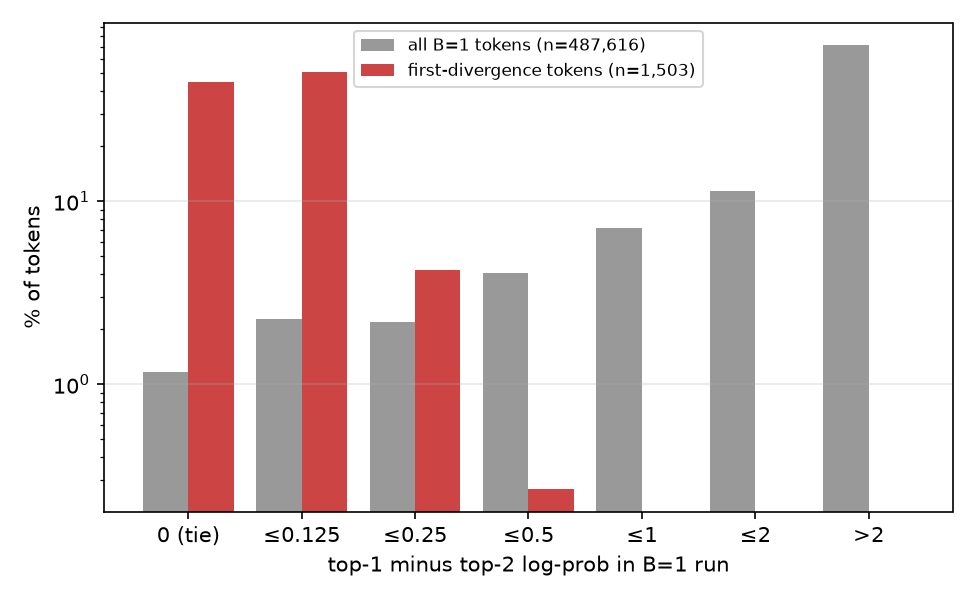
\includegraphics[width=\textwidth]{figures/margin_at_divergence.png}
        \caption{Margin distribution (bf16, log scale)}
        \label{fig:margin}
    \end{subfigure}
    \hfill
    \begin{subfigure}[b]{0.49\textwidth}
        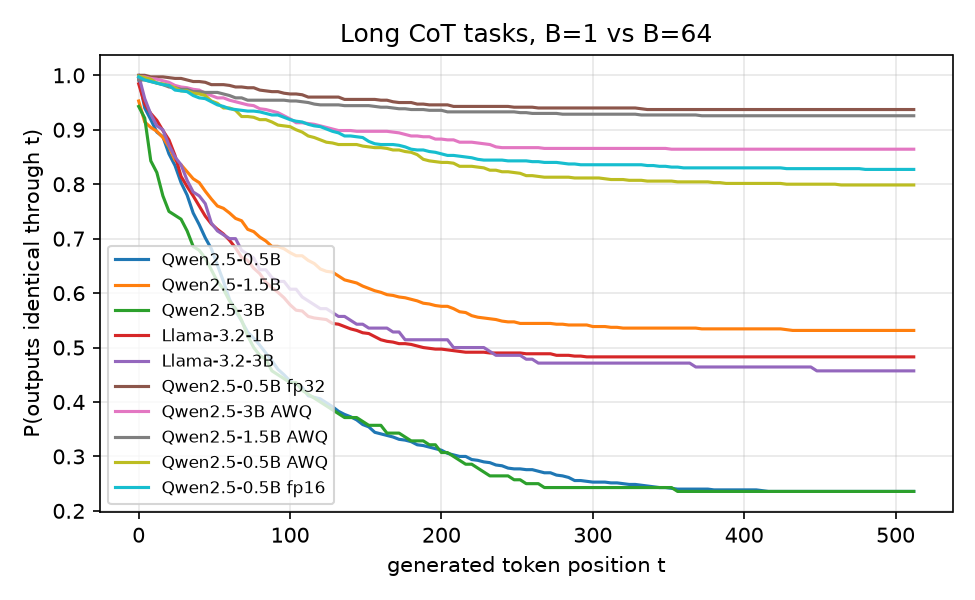
\includegraphics[width=\textwidth]{figures/survival_identical_prefix.png}
        \caption{Identical-prefix survival (CoT tasks)}
        \label{fig:survival}
    \end{subfigure}
    \caption{\captiona Top-1 minus top-2 log-probability in the $B=1$ run for all generated tokens (gray, $n=487{,}616$) and for first-divergence tokens (red, $n=1{,}503$). Divergences sit almost entirely at exact ties or within one bf16 step (0.125 nats), and never at margins above 0.5. \captionb Probability that the $B=1$ and $B=64$ outputs are still identical after $t$ generated tokens. bf16 curves drop steeply in the first 100--200 tokens and level off at 24--53\%; fp32 stays above 93\%.}
    \label{fig:mech}
\end{figure}

{\bf Every bf16 divergence starts at a near-tie.} bf16 stores logits with an 8-bit significand, so log-probabilities near the top of the distribution fall on a grid with steps of 0.0625--0.125 nats. Only about 1\% of all generated tokens are exact top-2 ties. Yet 43--47\% of first-divergence tokens are exact ties, a roughly 40$\times$ enrichment, and 91--100\% lie within one rounding step (\tabref{tab:mechanism}, \figref{fig:margin}). The largest margin at any divergence was 0.375 nats for bf16 and 0.047 nats for fp16 and fp32. Batch-dependent reduction order perturbs the logits by about one rounding step, which is enough to flip the argmax only where two candidates are (nearly) tied.

{\bf Precision controls the rate.} On identical \qwen-0.5B weights, the share of prompts that diverge between $B=1$ and $B=64$ falls monotonically from 33.5\% (bf16) to 7.3\% (fp16) and 2.8\% (fp32). Finer formats produce fewer ties (0.14\% of tokens in fp16, essentially none in fp32), and their divergences occur at much smaller margins (median 0.016 and 0.0014 nats). The AWQ models store 4-bit weights but compute in fp16, and they diverge at the fp16 level (3--8\%), well below their bf16 counterparts. So activation precision, not weight quantization, sets the rate.

\para{Divergences do not re-synchronize.} Once two runs choose different tokens at a near-tie, their continuations differ for the rest of the output (\figref{fig:survival}). For bf16, the median first divergence in CoT outputs is 45--57 tokens in, at 20--40\% of the output length (60--110 tokens for fp16, fp32 and AWQ). For bf16 short-label tasks, 44--100\% of divergences occur at the very first generated token, which is decided by the prefill pass.

\subsection{Length versus task type}
\label{sec:res_length}

\begin{figure}[t]
    \centering
    \begin{subfigure}[b]{0.40\textwidth}
        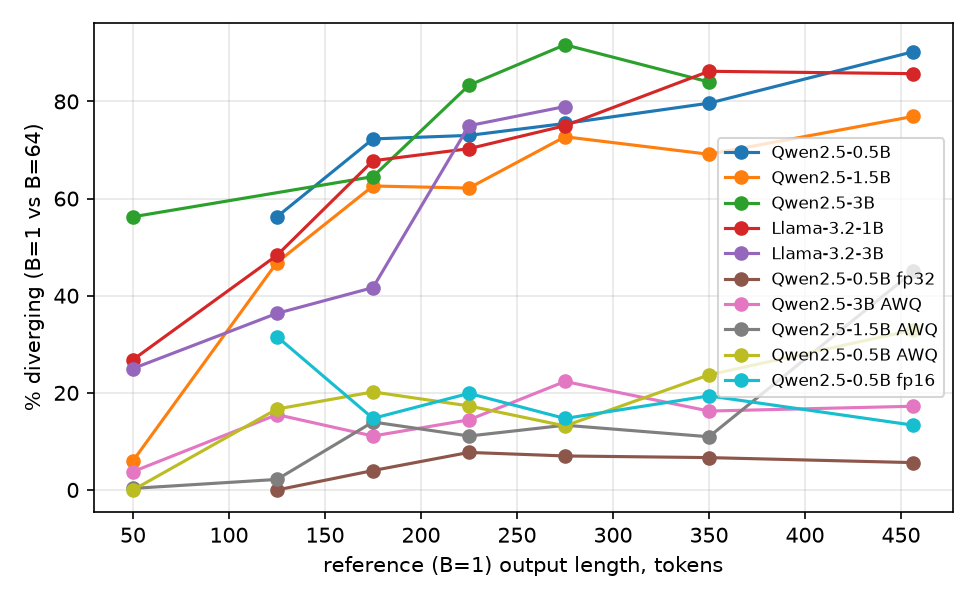
\includegraphics[width=\textwidth]{figures/divergence_vs_length.png}
        \caption{Divergence vs.\ output length (CoT)}
        \label{fig:length}
    \end{subfigure}
    \hfill
    \begin{subfigure}[b]{0.58\textwidth}
        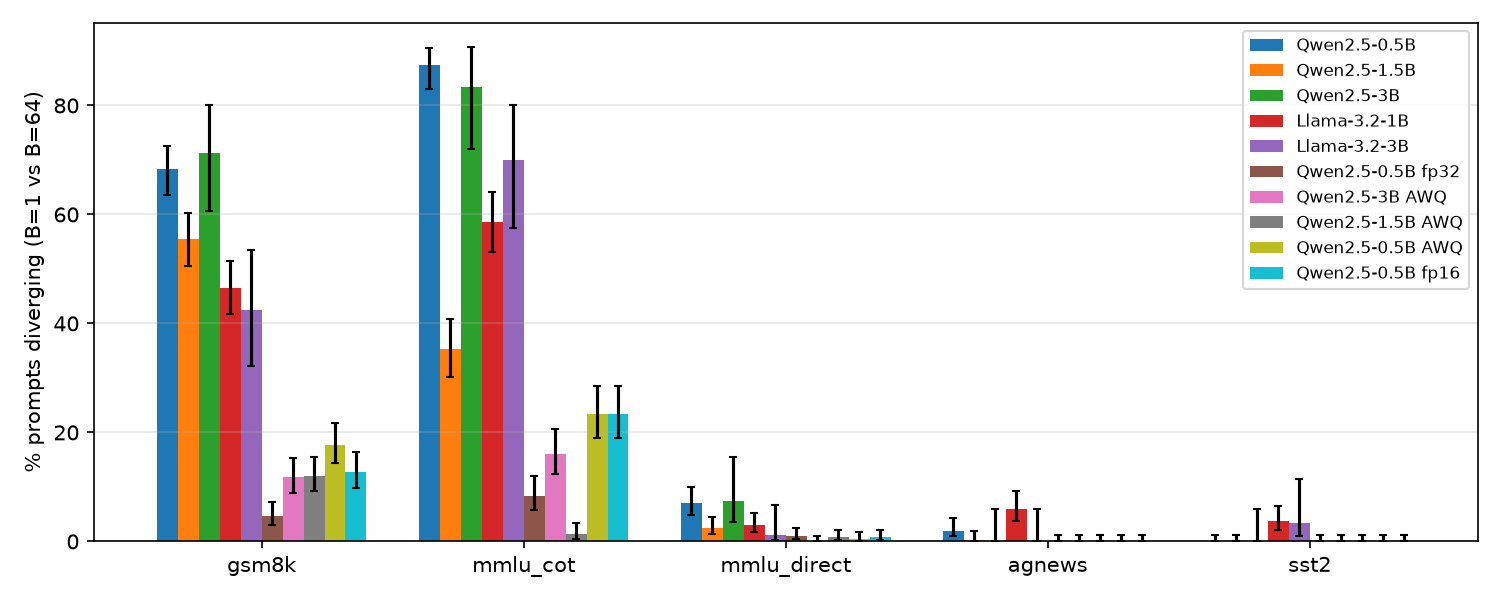
\includegraphics[width=\textwidth]{figures/divergence_by_task.png}
        \caption{Divergence by task}
        \label{fig:task}
    \end{subfigure}
    \caption{\captiona Share of CoT prompts that diverge ($B=1$ vs $B=64$), binned by the length of the $B=1$ output (bins with $\ge$10 items). bf16 divergence rises from 6--56\% for $\sim$50-token outputs to 77--90\% beyond 400 tokens. \captionb Divergence by task with Wilson 95\% CIs. Label tasks look stable, but their outputs are only 1--3 tokens long; per token they are not more stable (\secref{sec:res_length}).}
    \label{fig:lengthtask}
\end{figure}

{\bf H2 is supported: longer outputs diverge more.} Each generated token is another chance to hit a near-tie, so divergence rises steeply with output length (\figref{fig:length}). In a logistic regression on CoT items ($B=1$ vs $B=64$, all models), the coefficient on log length is $+1.14$ ($p\approx10^{-78}$). Across all tasks it is $+0.95$ ($p\approx10^{-67}$).

{\bf H3 is refuted as stated: the task effect is a length effect.} Classification looks far more stable than CoT (1--4\% vs 47--76\%, \figref{fig:task}), but its outputs are only 1--3 tokens long. Once log length is in the regression, the coefficient for short-label vs CoT is $-0.14$ with $p=0.58$. The per-token hazard (divergences per 1,000 tokens at risk) is \emph{not} lower for label tasks. For bf16 models it is 3.7--5.8 for \gsm, 5.7--12.9 for \mmlucot, 5.8--36.6 for \mmludirect, and 0--31 for \agnews and \sst. The first token of an uncertain multiple-choice answer is especially prone to ties. Within CoT tasks, math diverges \emph{less} than knowledge questions: at equal length, \gsm has an odds ratio of 0.41 relative to \mmlucot ($p\approx5\times10^{-31}$). One plausible reading is that arithmetic steps have more peaked next-token distributions, and so fewer near-ties, than free-text explanations of answer options.

\subsection{Does accuracy change?}
\label{sec:res_acc}

\begin{table}[t]
    \centering
    \caption{Accuracy under sequential (\bone) and batched (\bsf) decoding. $\Delta$ is \bsf minus \bone with a paired bootstrap 95\% CI. Flips count items that go right$\to$wrong (R$\to$W) or wrong$\to$right (W$\to$R). $p$ is the exact McNemar test, with the Holm-adjusted value over 28 tests in parentheses. No difference is significant, but bf16 models flip 3--5\% of items. 3B bf16 models use the 340-item subset. Lowest flip rate in \textbf{bold}.}
    \label{tab:accuracy}
    \resizebox{\textwidth}{!}{%
    \begin{tabular}{@{}llccccccc@{}}
        \toprule
        \textbf{Model} & \textbf{dtype} & \textbf{Acc \bone} & \textbf{Acc \bsf} & $\Delta$ (pp) [95\% CI] & \textbf{R$\to$W} & \textbf{W$\to$R} & \textbf{Flip \%} & $p$ (Holm) \\
        \midrule
        \qwen-0.5B & bf16 & 56.18 & 56.88 & $+0.71$ [$-0.41$, $+1.76$] & 39 & 51 & 5.3 & 0.25 (1.0) \\
        \qwen-1.5B & bf16 & 70.88 & 70.59 & $-0.29$ [$-1.06$, $+0.59$] & 29 & 24 & 3.1 & 0.58 (1.0) \\
        \qwen-3B   & bf16 & 72.94 & 71.76 & $-1.18$ [$-2.94$, $+0.59$] & 7 & 3 & 2.9 & 0.34 (1.0) \\
        \llama-1B  & bf16 & 50.12 & 49.94 & $-0.18$ [$-1.12$, $+0.76$] & 35 & 32 & 3.9 & 0.81 (1.0) \\
        \llama-3B  & bf16 & 67.65 & 69.41 & $+1.76$ [$-0.29$, $+4.12$] & 4 & 10 & 4.1 & 0.18 (1.0) \\
        \midrule
        \qwen-0.5B & fp16 & 56.82 & 56.82 & $\phantom{+}0.00$ [$-0.41$, $+0.47$] & 7 & 7 & 0.8 & 1.0 (1.0) \\
        \qwen-0.5B & fp32 & 56.35 & 56.12 & $-0.24$ [$-0.65$, $+0.18$] & 8 & 4 & 0.7 & 0.39 (1.0) \\
        \midrule
        \qwen-0.5B & AWQ & 45.00 & 45.24 & $+0.24$ [$-0.18$, $+0.65$] & 4 & 8 & 0.7 & 0.39 (1.0) \\
        \qwen-1.5B & AWQ & 67.47 & 67.35 & $-0.12$ [$-0.47$, $+0.18$] & 5 & 3 & 0.5 & 0.73 (1.0) \\
        \qwen-3B   & AWQ & 74.53 & 74.59 & $+0.06$ [$-0.18$, $+0.29$] & 2 & 3 & \textbf{0.3} & 1.0 (1.0) \\
        \bottomrule
    \end{tabular}
    }
\end{table}


\begin{figure}[t]
    \centering
    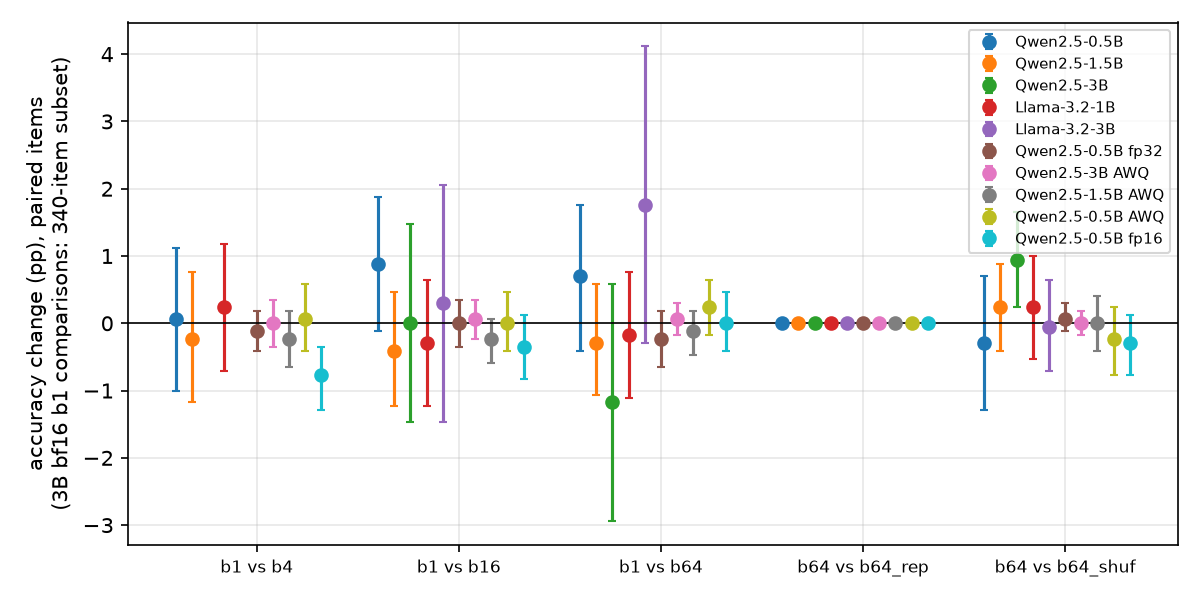
\includegraphics[width=0.85\linewidth]{figures/accuracy_delta.png}
    \caption{Paired accuracy change (percentage points) with bootstrap 95\% CIs for each comparison and model. Almost all intervals include zero, and no difference survives Holm correction; the identical-schedule repeat (\bsf vs \brep) is exactly zero. Changes reach $\pm$1--1.8\pp in single comparisons.}
    \label{fig:acc}
\end{figure}

{\bf H4 is supported: mean accuracy is robust, item correctness is not.} Across the five bf16 models, the mean absolute accuracy change between $B=1$ and $B=64$ is 0.8\pp, and no single change exceeds 1.8\pp (\tabref{tab:accuracy}, \figref{fig:acc}). None of the 28 primary tests is significant after Holm correction; the smallest raw $p$ is 0.002 (fp16, $B=1$ vs $B=4$, $-0.76$\pp), which becomes 0.066 after adjustment. Flips are symmetric (R$\to$W $\approx$ W$\to$R), so batching neither helps nor hurts on average. It re-rolls borderline items. Still, 2.9--5.3\% of all items flip correctness for bf16 models, and the rate is much higher on CoT multiple-choice: 16.3\% of \mmlucot items flip for \qwen-0.5B, 11.7\% for \llama-3B, 8.3\% for \qwen-3B and 7.7\% for \llama-1B. One exploratory comparison outside the pre-specified family is nominally significant (\qwen-3B, \bsf vs \bshuf, $+0.94$\pp, $p=0.014$ uncorrected). With 10 such shuffle tests, this is consistent with chance.

\para{Example.} On a \gsm item, \qwen-1.5B at $B=1$ writes ``Initially, Hunter counted 50 cars.'' while at $B=64$ it writes ``\ldots 50 cars \emph{in the parking lot}.'' The runs split at token 19, where the $B=1$ margin is exactly one bf16 step (0.125). The $B=1$ run then reasons to the correct answer (35), while the $B=64$ run adds an extra, wrong step and answers 55. More examples are in \appref{app:examples}.

\subsection{Does model size matter?}
\label{sec:res_size}

\begin{table}[t]
    \centering
    \small
    \caption{CoT divergence (\%) between \bsf and \bshuf ($n=700$) by model size. There is no monotone trend; \qwen-1.5B is the most stable size in both dtypes.}
    \label{tab:size}
    \begin{tabular}{@{}lccc@{}}
        \toprule
        & \textbf{0.5B / 1B} & \textbf{1.5B} & \textbf{3B} \\
        \midrule
        \qwen (bf16) & 72.7 & \textbf{40.0} & 63.7 \\
        \qwen (AWQ)  & 19.9 & \textbf{8.7}  & 13.9 \\
        \llama (bf16) & \textbf{45.3} (1B) & -- & 47.0 \\
        \bottomrule
    \end{tabular}
\end{table}

{\bf H5 is not supported.} We find no monotone relation between model size and divergence (Spearman $\rho=-0.05$, $p=0.93$ over the five bf16 models, CoT, $B=1$ vs $B=64$). \qwen-1.5B is the most stable \qwen model in both bf16 and AWQ, and \qwen-3B diverges about as often as 0.5B (\tabref{tab:size}). Size effects are small and model-specific, while dtype changes the rate by 5--15$\times$. Larger models also write different and often longer CoTs, which could confound the comparison, but the length bins in \figref{fig:length} show no consistent size ordering either.
